%%%%%%%%%%%%%%%%%%%%%%%%%%%%%%%%%%%%%%%%%
% Beamer Presentation
% LaTeX Template
% Version 1.0 (10/11/12)
%
% This template has been downloaded from:
% http://www.LaTeXTemplates.com
%
% License:
% CC BY-NC-SA 3.0 (http://creativecommons.org/licenses/by-nc-sa/3.0/)
%
%%%%%%%%%%%%%%%%%%%%%%%%%%%%%%%%%%%%%%%%%

%----------------------------------------------------------------------------------------
%	PACKAGES AND THEMES
%----------------------------------------------------------------------------------------

\documentclass{beamer}

\usepackage[utf8]{inputenc}

\mode<presentation> {

% The Beamer class comes with a number of default slide themes
% which change the colors and layouts of slides. Below this is a list
% of all the themes, uncomment each in turn to see what they look like.

%\usetheme{default}
%\usetheme{AnnArbor}
%\usetheme{Antibes}
%\usetheme{Bergen}
%\usetheme{Berkeley}
%\usetheme{Berlin}
%\usetheme{Boadilla}
%\usetheme{CambridgeUS}
%\usetheme{Copenhagen}
%\usetheme{Darmstadt}
%\usetheme{Dresden}
%\usetheme{Frankfurt}
%\usetheme{Goettingen}
%\usetheme{Hannover}
%\usetheme{Ilmenau}
%\usetheme{JuanLesPins}
%\usetheme{Luebeck}
\usetheme{Madrid}
%\usetheme{Malmoe}
%\usetheme{Marburg}
%\usetheme{Montpellier}
%\usetheme{PaloAlto}
%\usetheme{Pittsburgh}
%\usetheme{Rochester}
%\usetheme{Singapore}
%\usetheme{Szeged}
%\usetheme{Warsaw}

% As well as themes, the Beamer class has a number of color themes
% for any slide theme. Uncomment each of these in turn to see how it
% changes the colors of your current slide theme.

%\usecolortheme{albatross}
%\usecolortheme{beaver}
%\usecolortheme{beetle}
%\usecolortheme{crane}
%\usecolortheme{dolphin}
%\usecolortheme{dove}
%\usecolortheme{fly}
%\usecolortheme{lily}
%\usecolortheme{orchid}
%\usecolortheme{rose}
%\usecolortheme{seagull}
%\usecolortheme{seahorse}
%\usecolortheme{whale}
%\usecolortheme{wolverine}

%\setbeamertemplate{footline} % To remove the footer line in all slides uncomment this line
%\setbeamertemplate{footline}[page number] % To replace the footer line in all slides with a simple slide count uncomment this line

%\setbeamertemplate{navigation symbols}{} % To remove the navigation symbols from the bottom of all slides uncomment this line
}

\usepackage{graphicx} % Allows including images
\usepackage{booktabs} % Allows the use of \toprule, \midrule and \bottomrule in tables
\usepackage{listings}                   % para formatar código-fonte (ex. em Java)
\usepackage{xspace}
\usepackage{color}

\newcommand\adhoc{\emph{ad-hoc}\xspace}
\newcommand\sectiontitle[1]{\begin{center}\huge\textbf{#1}\end{center}}
\newcommand\subtitulo[1]{{\large \textbf{#1}}}
\newcommand\frase[1]{\begin{center}\large#1\end{center}}

%----------------------------------------------------------------------------------------
%	TITLE PAGE
%----------------------------------------------------------------------------------------

\title[Defesa mestrado]{Implantação automatizada de composições de \\ serviços web de grande escala} % The short title appears at the bottom of every slide, the full title is only on the title page

\author{Leonardo Leite} % Your name
\institute[IME - USP] % Your institution as it will appear on the bottom of every slide, may be shorthand to save space
{
IME - USP \\ % Your institution for the title page
\medskip
%\textit{leofl@ime.usp.br} % Your email address
}
\date{26 de maio de 2014} % Date, can be changed to a custom date

\begin{document}

\begin{frame}
\titlepage % Print the title page as the first slide
\begin{center}
{\scriptsize
Orientador: Marco Aurélio Gerosa \\
Coorientador: Fabio Kon
}
\end{center}
\end{frame}

\begin{frame}
\frametitle{Conteúdo} % Table of contents slide, comment this block out to remove it
\tableofcontents % Throughout your presentation, if you choose to use \section{} and \subsection{} commands, these will automatically be printed on this slide as an overview of your presentation
\end{frame}

%----------------------------------------------------------------------------------------
%	PRESENTATION SLIDES
%----------------------------------------------------------------------------------------

%------------------------------------------------
\section{Conceitos} % Sections can be created in order to organize your presentation into discrete blocks, all sections and subsections are automatically printed in the table of contents as an overview of the talk
%------------------------------------------------

%\subsection{Subsection Example} % A subsection can be created just before a set of slides with a common theme to further break down your presentation into chunks



\begin{frame}
\frametitle{Implantação de sistemas}

\frase{O processo de implantação manual se torna moroso e propenso a erros,
principalmente na implantação de sistemas distribuídos.}

\end{frame}

%------------------------------------------------

\begin{frame}
\frametitle{Implantação de sistemas}

\subtitulo{Processo de implantação automatizada}

\begin{itemize}
\item Reprodutível
\item Confiável
\item Fácil de ser executado
\end{itemize}

\vspace{0.4cm}

\subtitulo{Abordagens}

\begin{itemize}
\item scripts vs especificação declarativa
\item \adhoc vs baseadas em middleware
\end{itemize}


\end{frame}

%------------------------------------------------

\begin{frame}
\frametitle{Composições de serviços web}

\begin{itemize}
\item Interfaces acessíveis por máquinas
\item Automação de fluxos de negócios
\item Coreografias
\end{itemize}

\begin{figure}
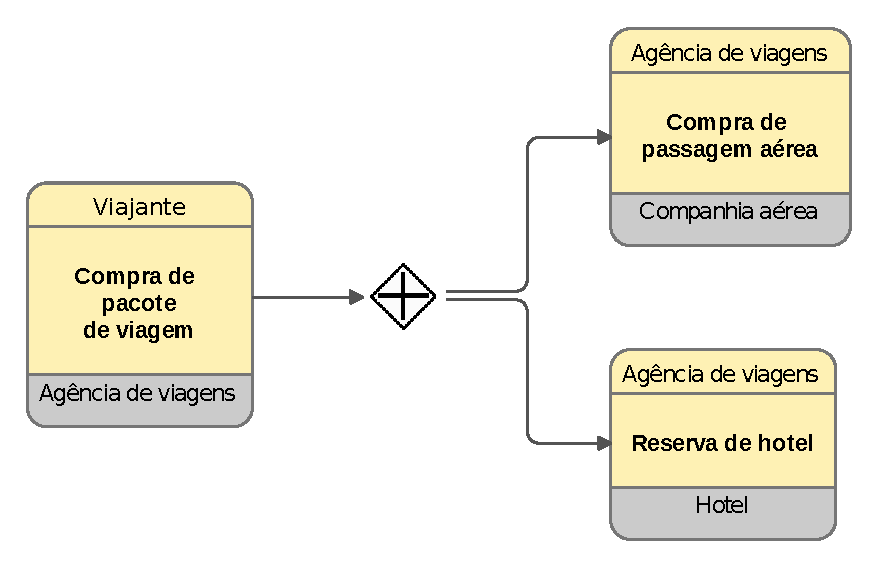
\includegraphics[width=0.7\linewidth]{img/bpmn2}
\end{figure}


\end{frame}

%------------------------------------------------

\begin{frame}
\frametitle{Composições de serviços web}

\begin{figure}
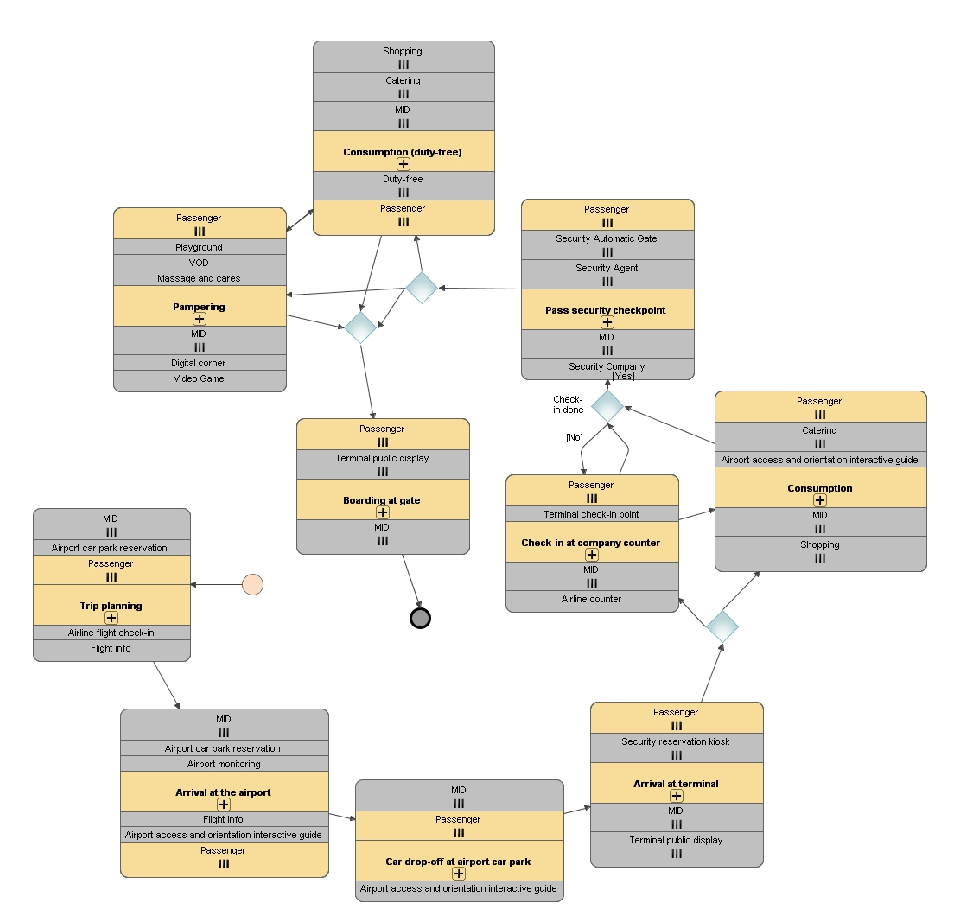
\includegraphics[width=0.7\linewidth]{img/chorwp6}
\end{figure}


\end{frame}

%------------------------------------------------

\begin{frame}
\frametitle{Desafios na implantação em grande-escala}

\begin{itemize}
\item Processo
\item Falhas
\item Disponibilidade
\item Escalabilidade
\item Heterogeneidade
\item Múltiplas organizações
\item Adaptabilidade
\end{itemize}

\end{frame}

%------------------------------------------------

\begin{frame}
\frametitle{Virtualização e nuvem na implantação}

\begin{itemize}
\item Torna implantação facilmente reprodutível
\item Endereços dos nós desconhecidos antes da implantação
\item Servidores são efêmeros
\end{itemize}


\end{frame}

%------------------------------------------------

\section{Definição da pesquisa}

\begin{frame}

\sectiontitle{Definição da pesquisa}

\end{frame}

%------------------------------------------------

\begin{frame}
\frametitle{Contexto}

\frase{Composições de serviços web de grande escala.}

\end{frame}

%------------------------------------------------
\begin{frame}
\frametitle{Questão}

\frase{O quanto e como soluções de implantação \\ baseadas em middleware  
trazem benefícios nesse \\ contexto 
quando confrontadas com soluções \adhoc?}

\end{frame}

%------------------------------------------------

\begin{frame}
\frametitle{Objetivo}

\frase{Projetar, implementar e avaliar um middleware que forneça \\ suporte à implantação automatizada de  composições de \\ serviços web de grande escala.}

\end{frame}

%------------------------------------------------

\section{Trabalhos relacionados}

\begin{frame}

\sectiontitle{Trabalhos relacionados}

\end{frame}

%------------------------------------------------

\begin{frame}
\frametitle{Trabalhos relacionados}

{\small 
\begin{table}[!t]
\begin{center}
    \begin{tabular}{l c c c c c c}
	 \hline
	 \itshape{Trabalho} & \itshape{ADL} & \itshape{Escala} & \itshape{Composições} & \itshape{Nuvem} & \itshape{Heterog.} \\ \hline
    Chef & x  & - & - & - & - \\
    Capistrano & x  & - & - & - & - \\
    Nix & x  & x & \checkmark & x  & - \\
    Darwin/Regis & \checkmark  & x & \checkmark & x & x \\
    Olan & \checkmark & x & \checkmark & x & x  \\
    Quema et al. & \checkmark & \checkmark & \checkmark & x & x \\
    J2EE app deployment & \checkmark & x & \checkmark & x & x \\
    Globus Toolkit & \checkmark & x & \checkmark & x & x \\
    Dynasoar & - & x & x & x & ? \\
    Open Knowledge  & \checkmark & x & \checkmark & x & x \\
    TOSCA & \checkmark & x & \checkmark & \checkmark & \checkmark \\
	Juju & - & x & x & \checkmark & \checkmark \\
    Cloud Foundry & - & ? & x & \checkmark & \checkmark \\
    \textbf{Enactment Engine}   & \checkmark & \checkmark & \checkmark & \checkmark & \checkmark \\
    \end{tabular}
\end{center}
\end{table}
}

\end{frame}

%------------------------------------------------

\section{O CHOReOS Enactment Engine}

\begin{frame}

\sectiontitle{O CHOReOS Enactment Engine}

\end{frame}

%------------------------------------------------

\begin{frame}
\frametitle{O EE e os modelos de computação nuvem}

\begin{figure}
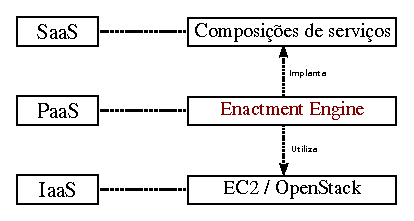
\includegraphics[width=1\linewidth]{img/nuvem_modelos}
\end{figure}

\end{frame}

%------------------------------------------------

\begin{frame}
\frametitle{Ambiente de execução do EE}

\begin{figure}
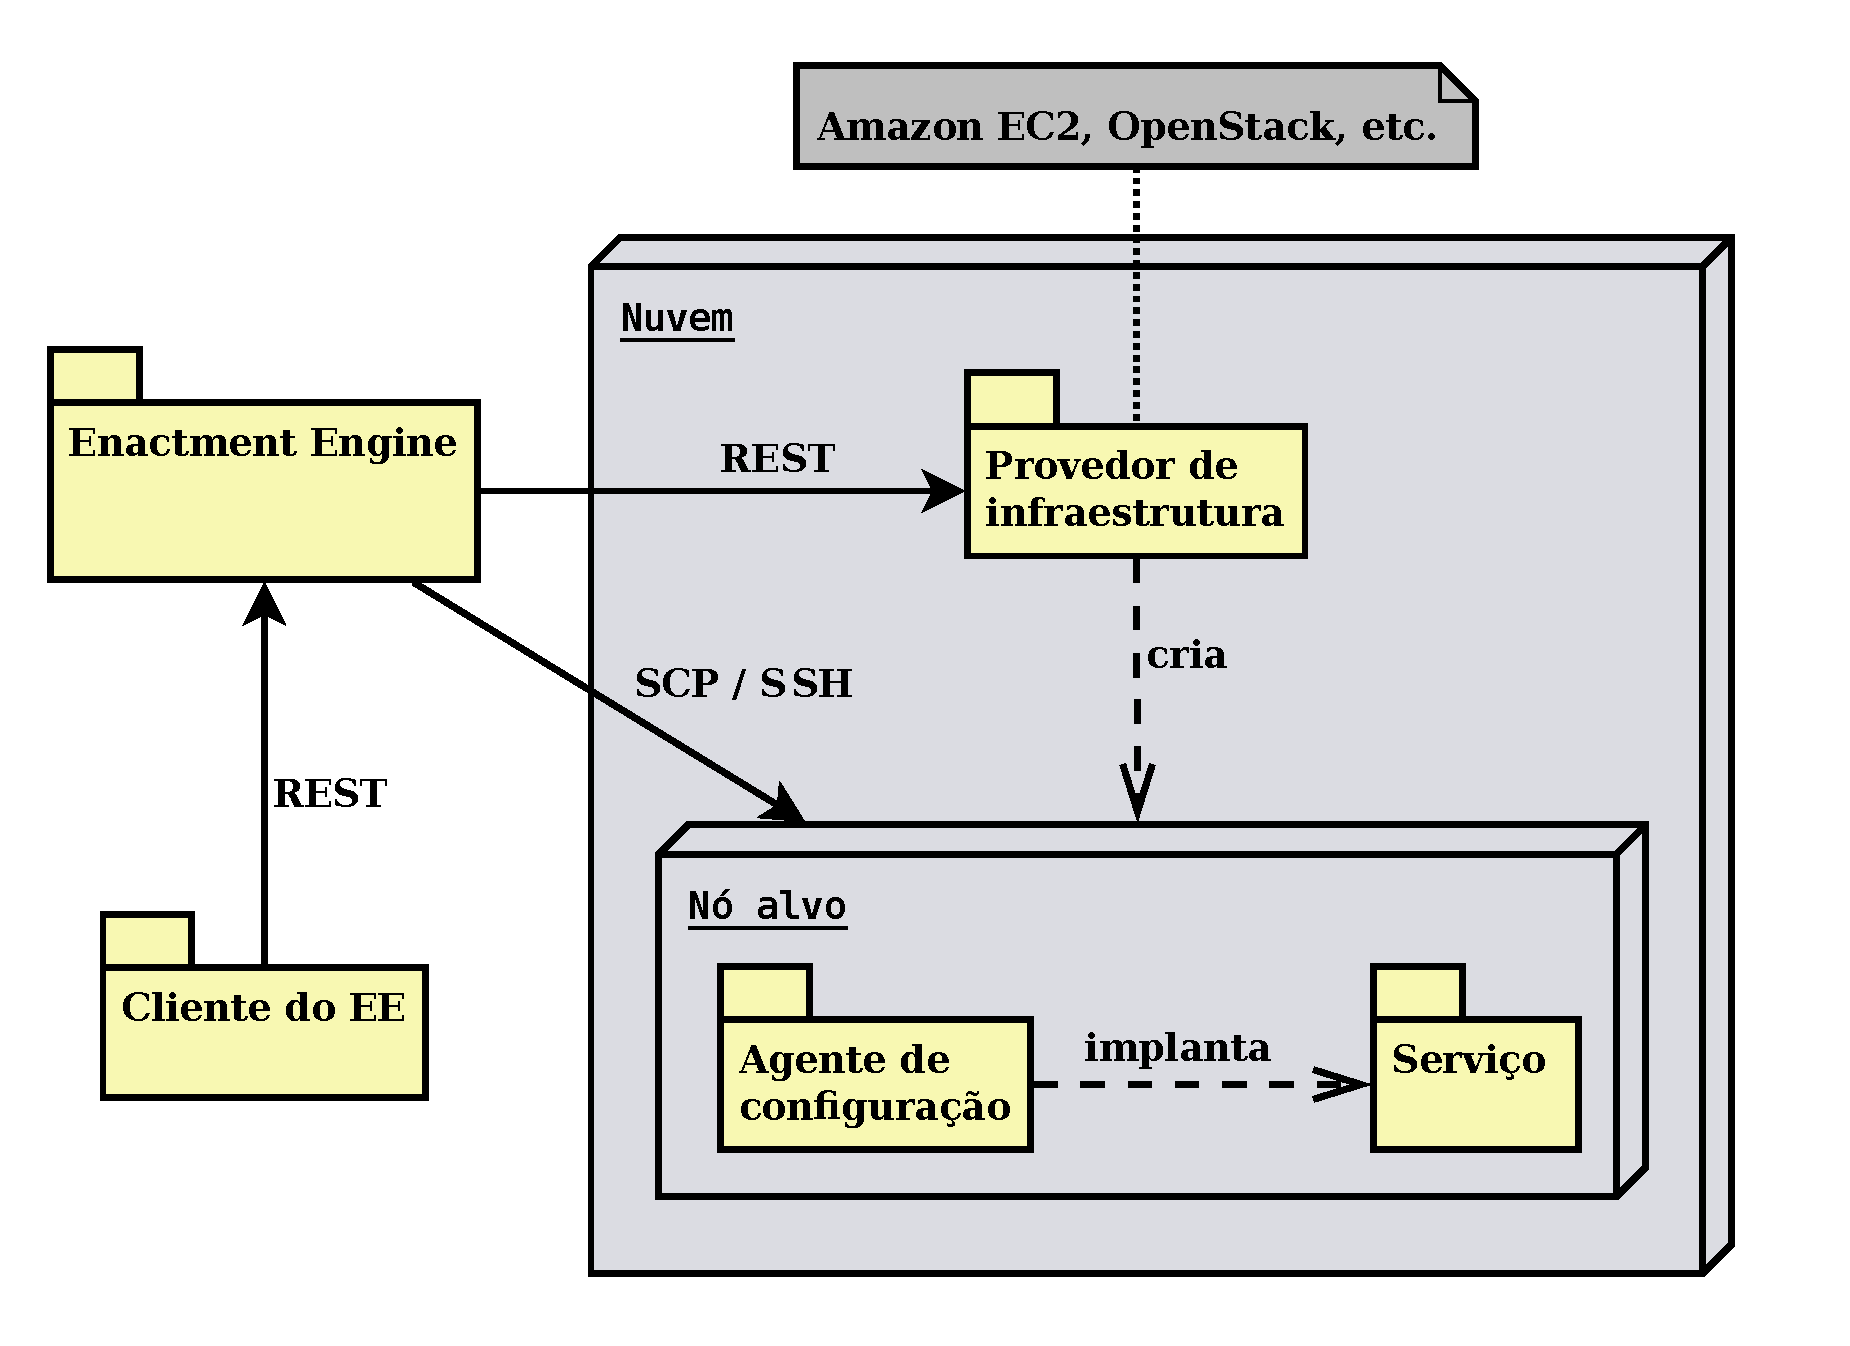
\includegraphics[width=0.8\linewidth]{img/arquitetura}
\end{figure}

\end{frame}

%------------------------------------------------

\begin{frame}
\frametitle{Estrutura da descrição arquitetural de uma coreografia}

\begin{figure}
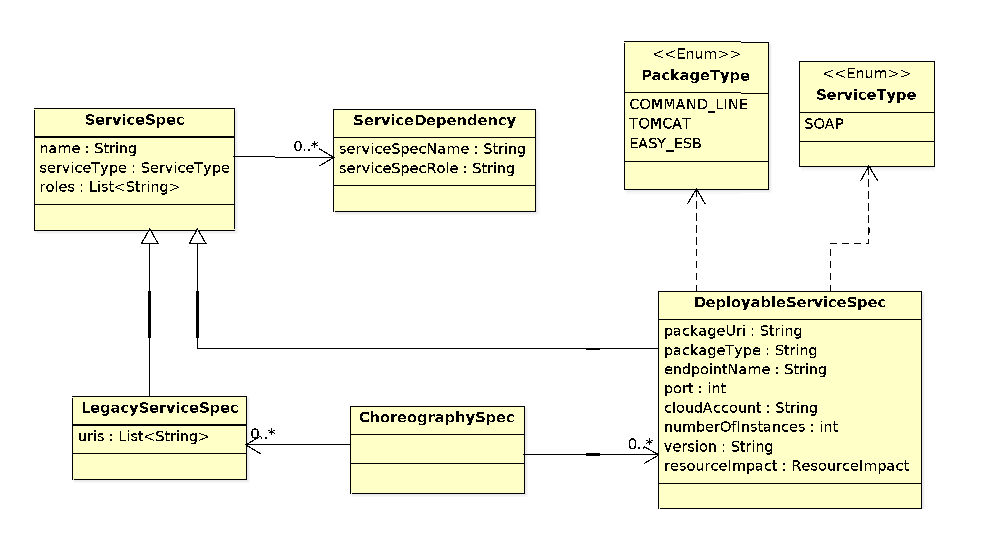
\includegraphics[width=1\linewidth]{img/chor_spec}
\end{figure}

\end{frame}

%------------------------------------------------

\begin{frame}[fragile]
\frametitle{Enlace entre serviços}

\begin{itemize}
\item Serviço $A$ depende de Serviço $B$
\item EE realiza a seguinte invocação ao Serviço $A$:
\end{itemize}

\begin{block}{}
\begin{lstlisting}
setInvocationAddress('Airline', 
                     'Nimbus Airline', 
                     ['http://nimbus.com/ws/' ])
\end{lstlisting}
\end{block}

\end{frame}

%------------------------------------------------

\begin{frame}
\frametitle{Processo de implantação implementado pelo EE}

\begin{figure}
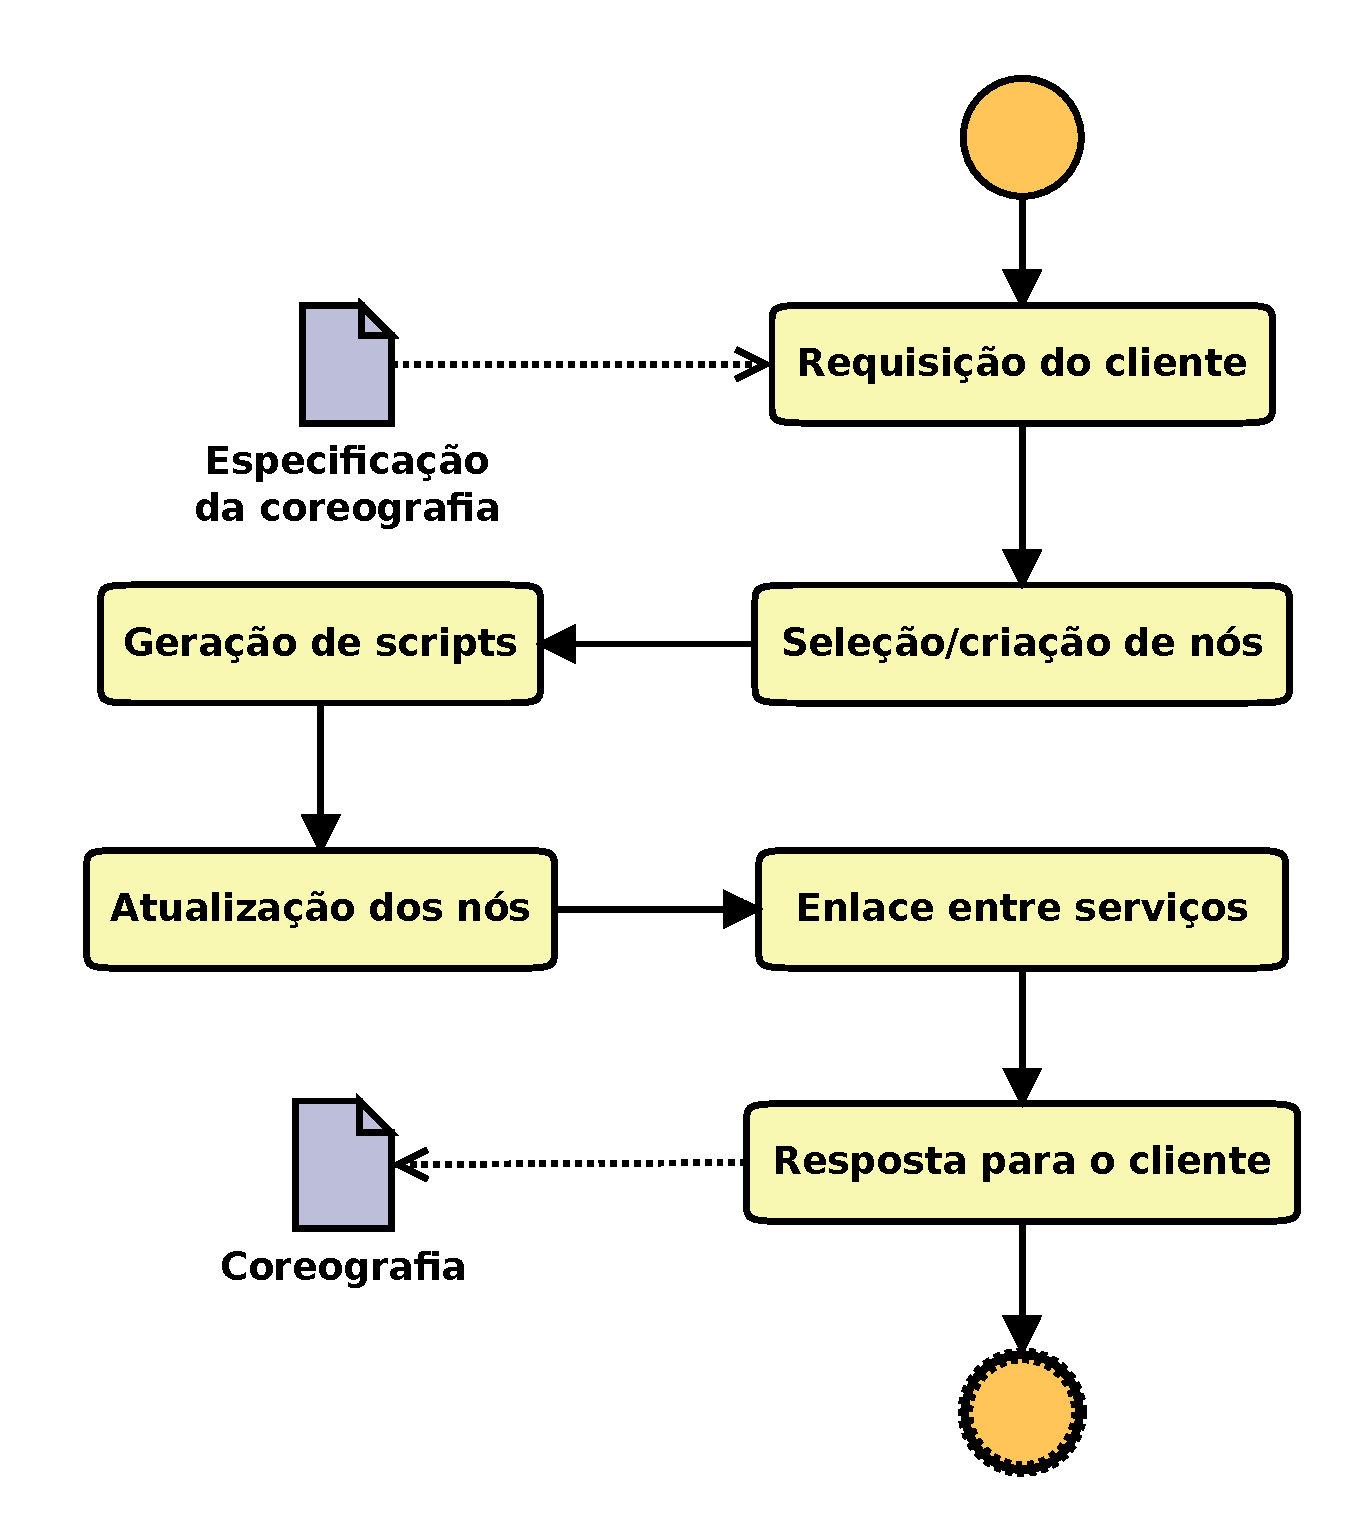
\includegraphics[width=0.55\linewidth]{img/processo}
\end{figure}

\end{frame}

%------------------------------------------------


\begin{frame}
\frametitle{O EE e os desafios de implantação em grande escala}

Como abordagens de implantação baseadas em middleware auxiliam o implantador em relação aos desafios listados?

\begin{itemize}
\item Processo
\item Falhas
\item Disponibilidade
\item Escalabilidade
\item Heterogeneidade
\item Múltiplas organizações
\item Adaptabilidade
\end{itemize}

\end{frame}


%------------------------------------------------

\begin{frame}
\frametitle{O EE e os desafios de implantação em grande escala}	

\subtitulo{Processo}

\vspace{1cm}

\begin{itemize}
\item Automação
\item Interface remota (REST)
\item Descrição declarativa
\item Infraestrutura virtualizada
\end{itemize}

\end{frame}


%------------------------------------------------

\begin{frame}
\frametitle{O EE e os desafios de implantação em grande escala}

\subtitulo{Falhas}

\vspace{1cm}

\begin{columns}[c]

\column{.45\textwidth}
\begin{itemize}
\item Invoker
\item Reservoir
\item Degradação suave
\item Idempotência
\end{itemize}

\column{.4\textwidth}
\begin{figure}
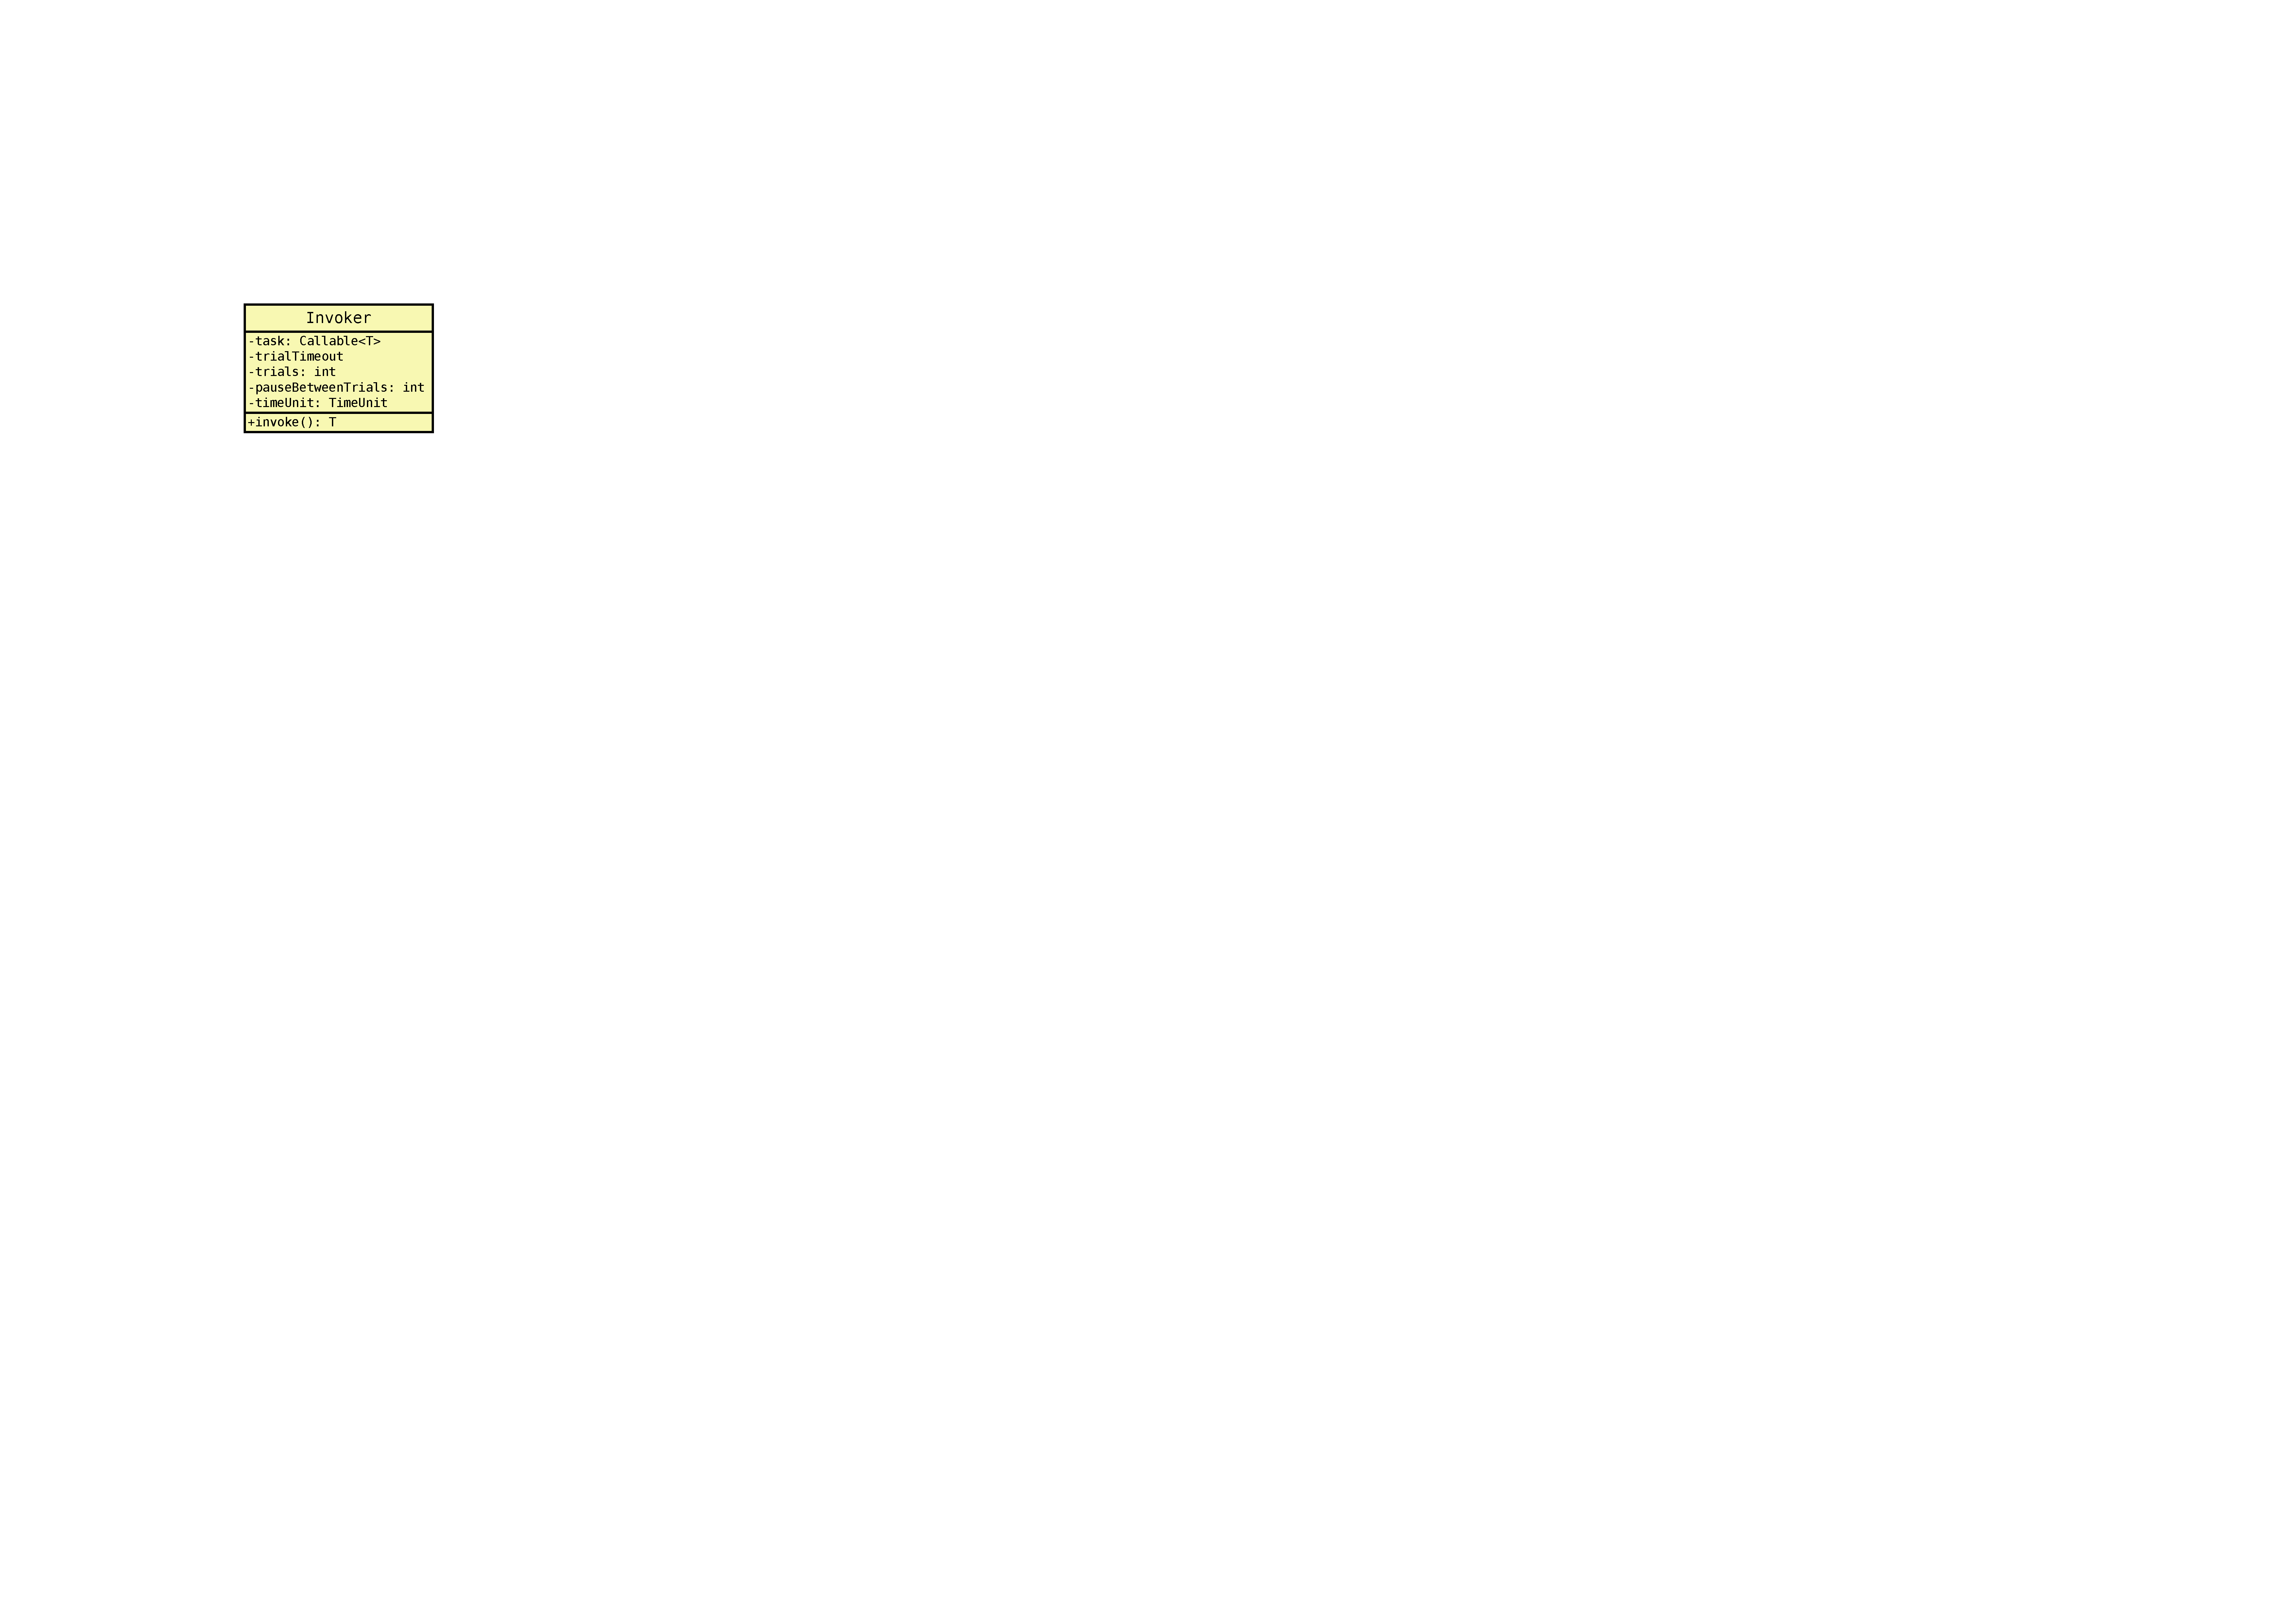
\includegraphics[width=0.8\linewidth]{img/invoker}
\end{figure}

\end{columns}
\end{frame}


%------------------------------------------------

\begin{frame}
\frametitle{O EE e os desafios de implantação em grande escala}

\subtitulo{Disponibilidade}

\vspace{1cm}

\begin{itemize}
\item Replicação
\item \textcolor{gray}{Dados}
\end{itemize}

\end{frame}


%------------------------------------------------

\begin{frame}
\frametitle{O EE e os desafios de implantação em grande escala}

\subtitulo{Escalabilidade}

\vspace{1cm}

\begin{itemize}
\item Concorrência (linguagem declarativa)
\item Tratamento de falhas
\item Evitar gargalos (Chef Server $\rightarrow$ Chef Solo)
\end{itemize}

\end{frame}


%------------------------------------------------

\begin{frame}
\frametitle{O EE e os desafios de implantação em grande escala}

\subtitulo{Heterogeneidade}

\vspace{1cm}

Pontos de extensão:

\begin{itemize}
\item Provedores de infraestrutura
\item Políticas de seleção de nós
\item Tipos de pacotes
\item Tipos de serviços
\end{itemize}

\end{frame}


%------------------------------------------------

\begin{frame}
\frametitle{O EE e os desafios de implantação em grande escala}

\subtitulo{Múltiplas organizações}

\vspace{1cm}

\begin{itemize}
\item Serviços legados
\item Implantação multi-nuvem
\item \textcolor{gray}{Federação}
\end{itemize}

\end{frame}


%------------------------------------------------

\begin{frame}
\frametitle{O EE e os desafios de implantação em grande escala}

\subtitulo{Adaptabilidade}

\vspace{1cm}

\begin{itemize}
\item Atualização das composições
\item Migração de serviços
\item Replicação de serviços
\item Implantação de infraestrutura de monitoramento
\end{itemize}

\end{frame}


%------------------------------------------------

\section{Avaliação}

\begin{frame}

\sectiontitle{Avaliação}

\end{frame}

%------------------------------------------------


\begin{frame}
\frametitle{Comparação EE vs \adhoc}

\begin{block}{EE}
\begin{itemize}
\item Desenvolvimento: 45 min
\item Execução: 4 min
\item Tamanho: 180 LoC Java
\end{itemize}
\end{block}

\vspace{0.6cm}

\begin{block}{\adhoc}
\begin{itemize}
\item Desenvolvimento: 9 horas
\item Execução: 60 min
\item Tamanho: 100 LoC Shell Script, 220 LoC Java, e 85 LoC Ruby
\end{itemize}
\end{block}

\end{frame}


%------------------------------------------------

\begin{frame}
\frametitle{Dificuldades da abordagem \adhoc}

\begin{itemize}
\item Muitas tecnologias
\item Passos manuais
\item Erros de digitação
\item Pouca paralelização
\end{itemize}

\vspace{0.5cm}

Solução \adhoc até poderia ficar melhor... \\
mas poderia ficar quase tão complexa quanto o próprio EE!


\end{frame}


%------------------------------------------------

\begin{frame}
\frametitle{Análise de desempenho}

\begin{table}
\centering
\begin{tabular}{r r r r c} \hline
\emph{Cenário} & \emph{Composições} & \emph{Tamanho} & \emph{Nós} & \emph{Serviços/Nós} \\ \hline
1 &  10 &  10 &  9 & 11 ou 12 \\
2 &  10 & 100 & 90 & 11 ou 12 \\
3 & 100 &  10 & 90 & 11 ou 12 \\
4 &  10 &  10 &  5 &       20 \\
\hline \end{tabular}
\end{table}

\end{frame}


%------------------------------------------------

\begin{frame}
\frametitle{Análise de desempenho}

\subtitulo{Topografia da composição sintética utilizada nos experimentos}

\begin{figure}
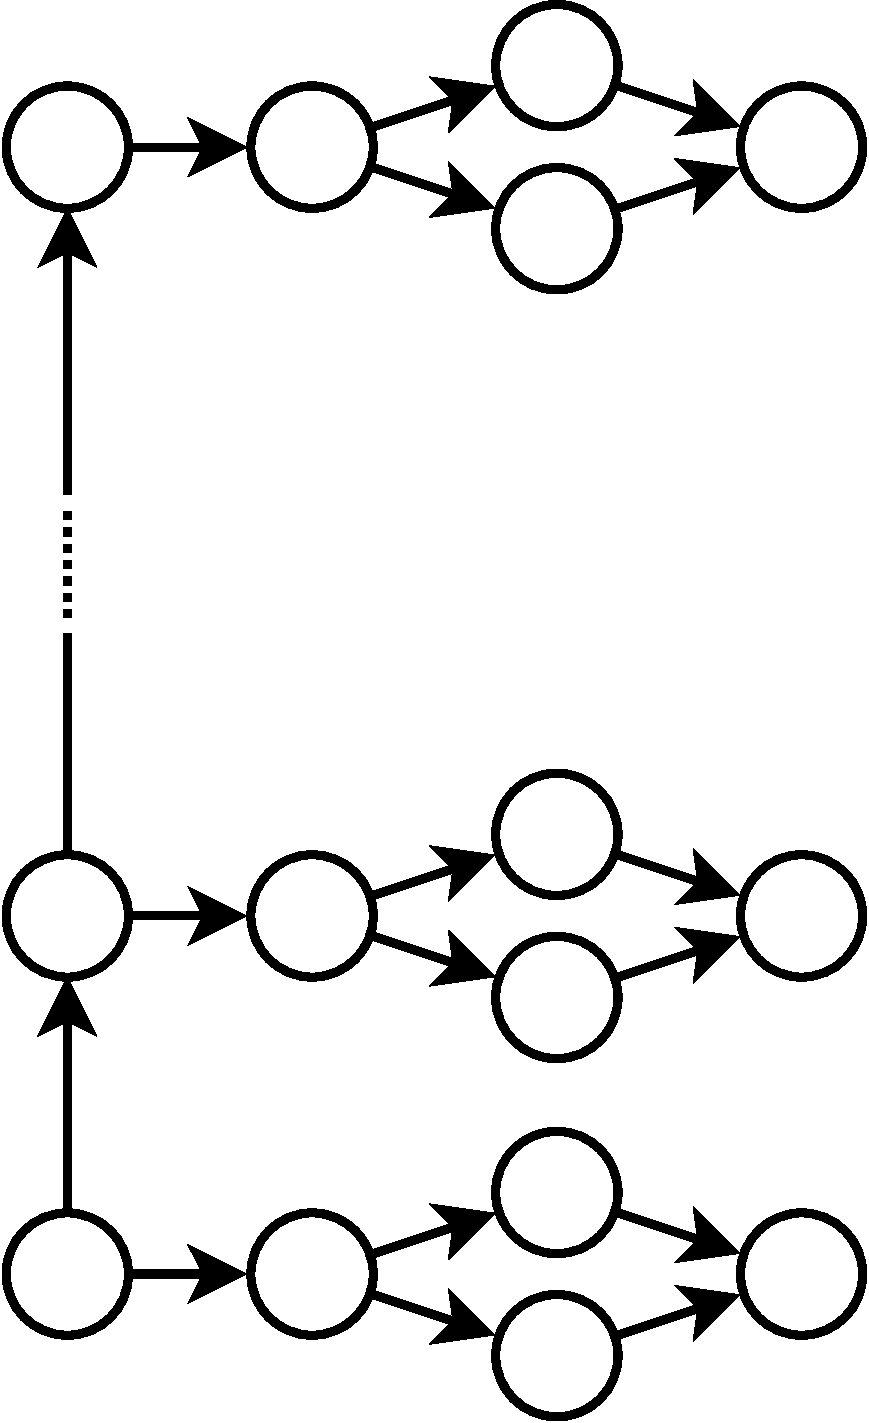
\includegraphics[width=0.35\linewidth, angle=270]{img/eval_composition}
\end{figure}

\end{frame}


%------------------------------------------------

\begin{frame}
\frametitle{Análise de desempenho}

\begin{table}
\centering
\begin{tabular}{c r@{ $\pm$ }l r@{ $\pm$ }l r@{ $\pm$ }l} \hline

\emph{Cenário} & \multicolumn{2}{c}{\emph{Tempo}} & \multicolumn{2}{c}{\emph{Composições}}   & \multicolumn{2}{c}{\emph{Serviços}}\\
                 & \multicolumn{2}{c}{(s)}           & \multicolumn{2}{c}{\emph{com sucesso}} & \multicolumn{2}{c}{\emph{com sucesso}}\\
\hline
1 &  467.9 &  34.8 & 10.0 & 0   & 100.0 & 0   (100\%) \\
2 & 1477.1 & 130.0 &  9.3 & 0.3 & 999.3 & 0.4 (99.9\%)\\
3 & 1455.2 & 159.1 & 98.9 & 0.8 & 998.5 & 1.3 (99.9\%)\\
4 &  585.2 &  38.1 & 10.0 & 0.1 & 100.0 & 0.1 (100\%)\\
\hline \end{tabular}
\end{table}

\end{frame}


%------------------------------------------------
\begin{frame}
\frametitle{Análise de escalabilidade}

\begin{figure}
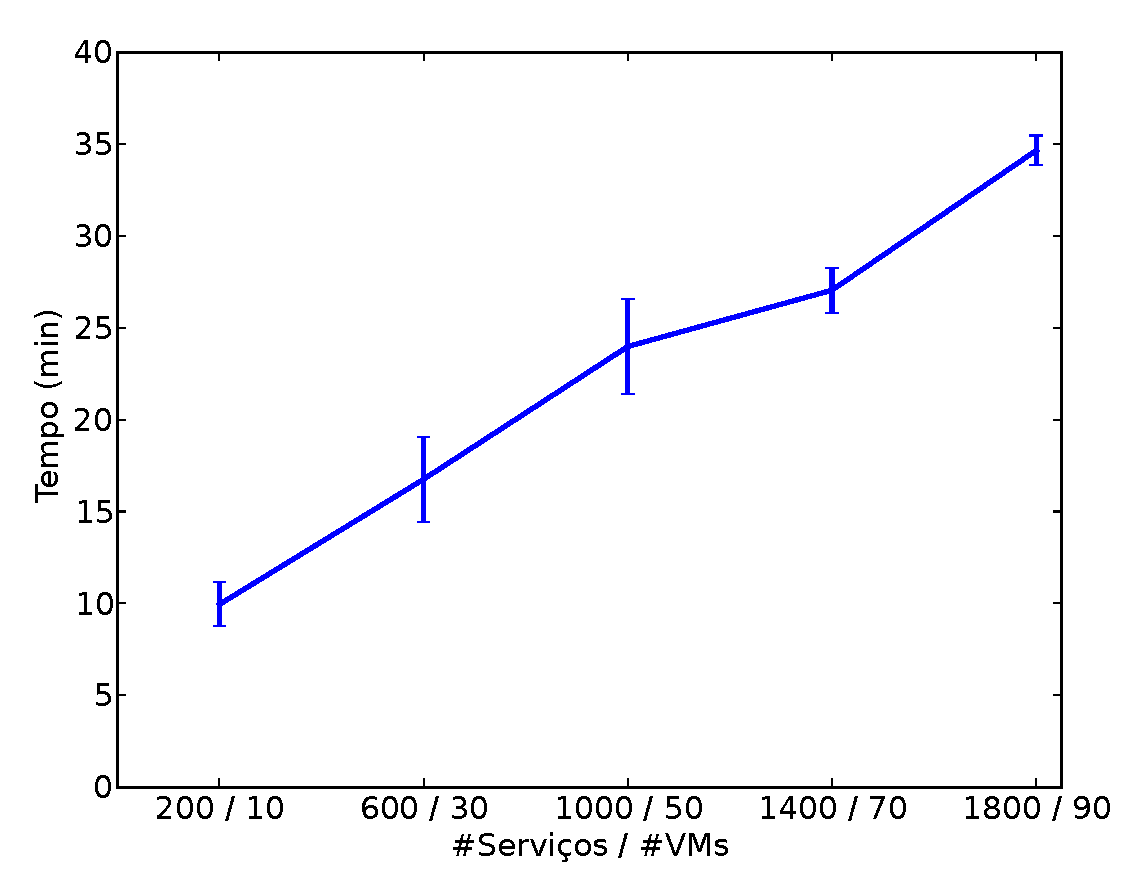
\includegraphics[width=0.8\linewidth]{img/scalability}
\end{figure}

\end{frame}


%------------------------------------------------
\begin{frame}
\frametitle{Efetividade do tratamento de falhas}

\begin{figure}
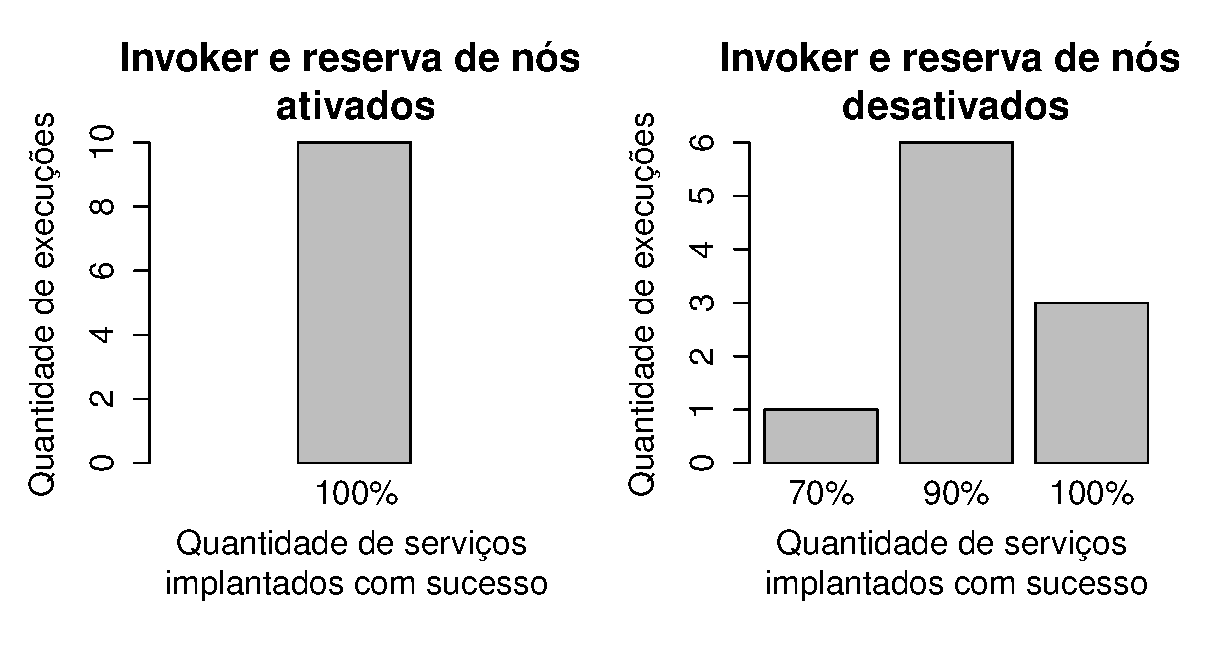
\includegraphics[width=0.9\linewidth]{img/error_handling}
\end{figure}

Cada execução: 1 composição de 100 serviços

\end{frame}


%------------------------------------------------

\section{Conclusões}

\begin{frame}

\sectiontitle{Conclusões}

\end{frame}

%------------------------------------------------


\begin{frame}
\frametitle{Contribuições}

\begin{itemize}
\item A implementação de um middleware que possibilita a implantação automatizada de composições de serviços. 
\item Uma comparação, baseada na literatura e em evidências empíricas, entre soluções de implantação automatizada com abordagens \adhoc e baseadas em middleware.
\end{itemize}

\end{frame}

%------------------------------------------------


\begin{frame}
\frametitle{Publicações}

{\small
\begin{block}{SBRC}
Leonardo Leite, Nelson Lago, Marco Aurélio Gerosa e Fabio Kon. Um Middleware para Encenação Automatizada de Coreografias de Serviços Web em Ambientes de Computação em Nuvem. Em \emph{31º Simpósio Brasileiro de Redes de Computadores e Sistemas Distribuídos}, 2013.
\end{block}

\begin{block}{MiniPlop Brasil}
Leonardo Leite. Fábrica dinâmica de dublês: testando classes que possuem dependências não injetáveis. Em \emph{Miniconferência Latino-Americana de Linguagens de Padrões para Programação}, 2013.
\end{block}

\begin{block}{SOCA}
Leonardo Leite, Gustavo Oliva, Guilherme Nogueira, Marco Aurélio Gerosa, Fabio Kon e Dejan Milojicic. A systematic literature review of service choreography adaptation. \emph{Service Oriented Computing and Applications}, 3(7):201--218, 2013.
\end{block}
}

\end{frame}

%------------------------------------------------

\begin{frame}
\frametitle{Trabalhos futuros}

\begin{itemize}
\item Análise multivariável de fatores que influenciam a escalabilidade
\item Experimentos com desenvolvedores
\item Algoritmos adaptativos para tratamento de falhas
\item Federação de instâncias do EE
\item Utilização de um balanceador de carga
\item Utilização de um barramento de serviços
\item Atualização dinâmica de composições de serviços
\end{itemize}

\end{frame}

%------------------------------------------------

\begin{frame}

{\Huge \centerline{Obrigado! }}

\vspace{1cm}

\textbf{Leonardo Alexandre Ferreira Leite} \\
\url{http://www.ime.usp.br/~leofl} \\
\url{leofl@ime.usp.br} \\

\vspace{0.6cm}

\textbf{CHOReOS Enactment Engine} \\
\url{http://ccsl.ime.usp.br/EnactmentEngine} \\
\url{https://github.com/choreos/enactment_engine}
\end{frame}

%----------------------------------------------------------------------------------------

\end{document} 